\documentclass{article}

\usepackage{fancyhdr}
\usepackage{extramarks}
\usepackage{amsmath}
\usepackage{amsthm}
\usepackage{amsfonts}
\usepackage{tikz}
\usepackage[plain]{algorithm}
\usepackage{algpseudocode}
\usepackage{enumerate}
\usepackage{amssymb}
\usepackage[margin=1in]{geometry}

\newcommand{\st}{~\mid~}
\newcommand{\ind}{$~~~$}
\usepackage{xcolor}

\graphicspath{ {./../images} }

\usetikzlibrary{automata,positioning,arrows}

%
% Basic Document Settings
%

\topmargin=-0.45in
\evensidemargin=0in
\oddsidemargin=0in
\textwidth=6.5in
\textheight=9.0in
\headsep=0.25in

\linespread{1.1}

\pagestyle{fancy}
\lhead{\hmwkAuthorName}
\chead{\hmwkClass:\ \hmwkTitle}
\rhead{\firstxmark}
\lfoot{\lastxmark}
\cfoot{\thepage}

\renewcommand\headrulewidth{0.4pt}
\renewcommand\footrulewidth{0.4pt}

\setlength\parindent{0pt}
\setlength{\parskip}{5pt}

%
% Create Problem Sections
%

\newcommand{\enterProblemHeader}[1]{
    \nobreak\extramarks{}{Problem \arabic{#1} continued on next page\ldots}\nobreak{}
    \nobreak\extramarks{Problem \arabic{#1} (continued)}{Problem \arabic{#1} continued on next page\ldots}\nobreak{}
}

\newcommand{\exitProblemHeader}[1]{
    \nobreak\extramarks{Problem \arabic{#1} (continued)}{Problem \arabic{#1} continued on next page\ldots}\nobreak{}
    \stepcounter{#1}
    \nobreak\extramarks{Problem \arabic{#1}}{}\nobreak{}
}

\setcounter{secnumdepth}{0}
\newcounter{partCounter}
\newcounter{homeworkProblemCounter}
\setcounter{homeworkProblemCounter}{1}
\nobreak\extramarks{Problem \arabic{homeworkProblemCounter}}{}\nobreak{}

%
% Homework Problem Environment
%
% This environment takes an optional argument. When given, it will adjust the
% problem counter. This is useful for when the problems given for your
% assignment aren't sequential. See the last 3 problems of this template for an
% example.
%
\newenvironment{homeworkProblem}[1][-1]{
    \ifnum#1>0
        \setcounter{homeworkProblemCounter}{#1}
    \fi
    \section{Problem \arabic{homeworkProblemCounter}}
    \setcounter{partCounter}{1}
    \enterProblemHeader{homeworkProblemCounter}
}{
    \exitProblemHeader{homeworkProblemCounter}
}

%
% Homework Details
%   - Title
%   - Due date
%   - Class
%   - Section/Time
%   - Instructor
%   - Author
%

\newcommand{\hmwkTitle}{Homework\ \#2}
\newcommand{\hmwkDueDate}{Apr 17, 2024}
\newcommand{\hmwkClass}{CSE 101}
\newcommand{\hmwkClassInstructor}{Professor Jones}
\newcommand{\hmwkAuthorName}{\textbf{Ray Tsai}}
\newcommand{\hmwkPID}{A16848188}

%
% Title Page
%

\title{
    \vspace{2in}
    \textmd{\textbf{\hmwkClass:\ \hmwkTitle}}\\
    \normalsize\vspace{0.1in}\small{Due\ on\ \hmwkDueDate\ at 23:59pm}\\
    \vspace{0.1in}\large{\textit{\hmwkClassInstructor}} \\
    \vspace{3in}
}

\author{
  \hmwkAuthorName \\
  \vspace{0.1in}\small\hmwkPID
}
\date{}

\renewcommand{\part}[1]{\textbf{\large Part \Alph{partCounter}}\stepcounter{partCounter}\\}

%
% Various Helper Commands
%

% Useful for algorithms
\newcommand{\alg}[1]{\textsc{\bfseries \footnotesize #1}}

% For derivatives
\newcommand{\deriv}[1]{\frac{\mathrm{d}}{\mathrm{d}x} (#1)}

% For partial derivatives
\newcommand{\pderiv}[2]{\frac{\partial}{\partial #1} (#2)}

% Integral dx
\newcommand{\dx}{\mathrm{d}x}

% Probability commands: Expectation, Variance, Covariance, Bias
\newcommand{\Var}{\mathrm{Var}}
\newcommand{\Cov}{\mathrm{Cov}}
\newcommand{\Bias}{\mathrm{Bias}}
\newcommand*{\Z}{\mathbb{Z}}
\newcommand*{\Q}{\mathbb{Q}}
\newcommand*{\R}{\mathbb{R}}
\newcommand*{\C}{\mathbb{C}}
\newcommand*{\N}{\mathbb{N}}
\newcommand*{\prob}{\mathds{P}}
\newcommand*{\E}{\mathds{E}}

\begin{document}

\maketitle

\pagebreak

\begin{homeworkProblem}
  Run the SCC algorithm on the following directed graph $G$. When doing DFS on $G^R$: whenever there
  is a choice of vertices to explore, always pick the one that is alphabetically first.\\
  {\scriptsize$
  A:  D,G\\
  B:  F,G,L\\
  C:  B,E\\
  D:  G,H\\
  E:  A,J\\
  F:  B\\
  G:  H\\
  H:  B,L\\
  I:  K\\
  J:  F,L\\
  K:  D\\
  L:  E,H,K$}
  \begin{enumerate}[(a)]
  \item In what order are the strongly connected components (SCCs) found?
  \begin{proof}
    We first run DFS on $G^R$ and get the {\fontfamily{qcr}\selectfont post} numbers:
    \begin{center}
      \begin{tabular}{|c|c|c|c|c|c|c|c|c|c|c|c|}
        \hline
        $A$ & $B$ & $C$ & $D$ & $E$ & $F$ & $G$ & $H$ & $I$ & $J$ & $K$ & $L$ \\
        \hline
        24 & 21 & 4 & 17 & 23 & 10 & 19 & 20 & 15 & 9 & 16 & 22 \\
        \hline
      \end{tabular}
    \end{center}
    Then, we run the undirected connected components algorithm on $G$ by descending
    {\fontfamily{qcr}\selectfont post} order:
    \begin{center}
      \begin{tabular}{|c|c|c|c|c|c|c|c|c|c|c|c|}
        \hline
        $A$ & $B$ & $C$ & $D$ & $E$ & $F$ & $G$ & $H$ & $I$ & $J$ & $K$ & $L$ \\
        \hline
        1 & 1 & 3 & 1 & 1 & 1 & 1 & 1 & 2 & 1 & 1 & 1 \\
        \hline
      \end{tabular}
    \end{center}
    Hence, we find the following strongly connected components in the following sequence:
    \[
      \{A, B, D, E, F, G, H, J, K, L\}, \{I\}, \{C\}.
    \]
  \end{proof}
  
  \item Which are source SCCs and which are sink SCCs?
  \begin{proof}
    Since $\{A, B, D, E, F, G, H, J, K, L\}$ does not have outgoing edges, it is a sink. Since SCCs
    $\{I\}$ and $\{C\}$ don't have incoming edges, they are sources. 
  \end{proof}
  
  \item Draw the ``metagraph" (each meta-node is an SCC of $G$)
  \begin{proof}
    The following is the metagraph of $G$, where node 1 represents $\{A, B, D, E, F, G, H, J, K,
    L\}$, node 2 represents $\{I\}$, and node 2 represents $\{C\}$.
    \begin{center}
      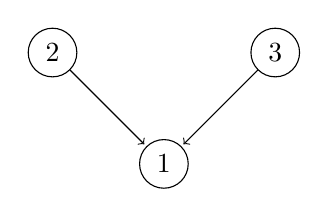
\begin{tikzpicture}[->, shorten >=1pt, auto, node distance=2cm, main node/.style={circle, draw}]

        \node[main node] (1) {1};
        \node[main node] (2) [above left of=1] {2};
        \node[main node] (3) [above right of=1] {3};
      
        \path[every node/.style={font=\sffamily\small}]
          (2) edge node [left] {} (1)
          (3) edge node [right] {} (1);
      \end{tikzpicture}
    \end{center}
  \end{proof}
  
  \end{enumerate}
\end{homeworkProblem}

\newpage

\begin{homeworkProblem}
  Consider the following problem:

\begin{quote}
Given a strongly connected simple \emph{directed} graph $G$, determine the total number of cycles in
the graph.

Consider the following algorithm that claims to compute the total number of cycles in the graph.
\end{quote}

For each algorithm, 
\begin{itemize}
\item
Provide a runtime analysis (Based on $|V|$ and $|E|$)
\item
identify if it correctly solves the problem.
\item
If it is correct, provide a correctness proof. If it is not correct, provide a counterexample.
\end{itemize}
\begin{enumerate}
\item
\begin{quote}
{\bf Algorithm1}($G$; a strongly connected simple directed graph $G$.)

\begin{enumerate}[1.]
\item
Run {\bf DFS}$(G)$
\item
c = 0
\item
{\bf for} each edge $(u,v)$ {\bf then}
\item
\ind {\bf if} $post(v) > post(u)$ {\bf then}
\item
\ind\ind $c = c + 1$
\item
{\bf return} c
\end{enumerate}
\end{quote}

\begin{proof}
  We first give a runtime analysis to this algorithm. We already know DFS takes $O(|V| + |E|)$ time.
  Following the DFS is a loop which iterates over all edges, which takes an additional $O(|E|)$
  time. Hence, the runtime complexity of this algorithm is $O(|V| + 2|E|) = O(|V| + |E|)$.

  However, the algorithm is incorrect. Consider the following graph:
  \begin{center}
    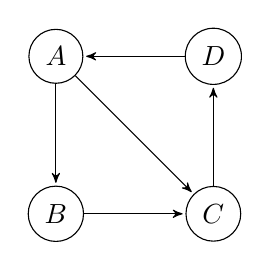
\begin{tikzpicture}[->, >=stealth', shorten >=1pt, auto, node distance=2cm, main node/.style={circle, draw}]

      \node[main node] (1) {$A$};
      \node[main node] (2) [right of=1] {$D$};
      \node[main node] (3) [below of=2] {$C$};
      \node[main node] (4) [below of=1] {$B$};
    
      \path[every node/.style={font=\sffamily\small}]
        (1) edge node [] {} (3)
        (2) edge node [] {} (1)
        (4) edge node [] {} (3)
        (1) edge node [] {} (4)
        (3) edge node [] {} (2);
    \end{tikzpicture}
  \end{center}
  Note that the graph is simple and strongly connected, as there is a directed hamiltonian cycle.
  Performing DFS on this graph starting from $A$ yields the following {\fontfamily{qcr}\selectfont
  post} numbers:
  \begin{center}
    \begin{tabular}{|c|c|c|c|}
      \hline
      $A$ & $B$ & $C$ & $D$ \\
      \hline
      8 & 7 & 6 & 5 \\
      \hline
    \end{tabular}
  \end{center}
  $(D, A)$ is the only edge that meets the condition at step 4, so the algorithm outputs 1. But then
  there are two cycles in the graph, namely $A \to C \to D \to A$ and $A \to B \to C \to D \to A$.
\end{proof}

\break

\item
\begin{quote}
{\bf Algorithm2}($G$; a strongly connected simple directed graph $G$.)

[[run graphsearch and every time you encounter a vertex you have already seen before, increment your
counter, $c$.]]

\begin{enumerate}[1.]
\item
$c = 0$
\item
{\bf for all} $v\in V$:
\item
\ind Status($v$) = {\bf U}
\item
Pick any vertex $s$
\item
Status($s$) = {\bf F}
\item
Initialize a Stack: $F = [s]$
\item
{\bf while} $|F| > 0$
\item
\ind $w = pop(F)$.
\item
\ind For each outgoing neighbor $y$ of $w$ (for each $(w,y)\in E$):
\item
\ind\ind {\bf if} Status($y$) $\neq$ {\bf U}:
\item
\ind\ind\ind $c = c+1$
\item
\ind\ind {\bf else:}
\item
\ind\ind\ind Status($y$) = {\bf F}
\item
\ind\ind\ind $push(F,y)$
\item
\ind Status($w$) = {\bf X}
\item
{\bf return} $c$
\end{enumerate}
\end{quote}
\end{enumerate}

\begin{proof}
  Since this algorithm is just graphsearch with a counter, the time complexity of the algorithm is
  the same as a standard graphsearch, which takes $O(|V| + |E|)$ time.

  However, this algorithm is incorrect. Consider the following graph:
  \begin{center}
    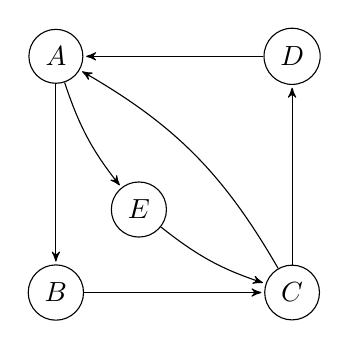
\begin{tikzpicture}[->, >=stealth', shorten >=1pt, auto, node distance=3cm, main node/.style={circle, draw}]

      \node[main node] (1) {$A$};
      \node[main node] (2) [right of=1] {$D$};
      \node[main node] (3) [below of=2] {$C$};
      \node[main node] (4) [below of=1] {$B$};
      \node[main node] (5) [below of=1, xshift=30,  yshift=30] {$E$};
    
      \path
      (3) edge [bend right=15] node {} (1)
      (1) edge [bend right=10] node {} (5)
      (5) edge [bend right=10] node {} (3)
      (2) edge node {} (1)
      (4) edge node {} (3)
      (1) edge node {} (4)
      (3) edge node {} (2);
    \end{tikzpicture}
  \end{center}
  The graph is obviously simple and strongly connected. We first note that the graph has 4 cycles, namely $A \to B \to C \to A$, $A
  \to B \to C \to D \to A$, $A \to E \to C \to A$, $A \to E \to C \to D \to A$.
  
  Suppose that the algorithm starts at vertex $A$. Here is the order of edges the for loop in
  the algorithm will check:
  \[
    (A, B) \to (A, E) \to (B, C) \to (C, \textbf{A}) \to (C, D) \to (D, \textbf{A}) \to (E, \textbf{C}).
  \]
  The bolded vertices represents the already visited vertices, which causes the counter to
  increment. But then the algorithm returns 3, which is not the number of cycles in the graph.
\end{proof}
\end{homeworkProblem}

\newpage

\begin{homeworkProblem}
  You are given a simple directed graph $G$ with vertex set $V$, edge set $E$ and vertex labels
  $L(v)\in  \{0,1\}$ as well as a starting and ending vertex $s,t$.

  Design a reasonably efficient algorithm that determines if there is a walk from $s$ to $t$ such
  that the sequence of vertex labels in the walk have exactly one occurrence of two 1's in a row.


  \begin{proof}
    Consider the following algorithm:
    \begin{quote}
      Create a graph $G'$ in the following way:

      for each vertex $v$ in $G$, create two copies $v', v''$ in $G'$. For each edge $(x, y)$ in
      $G$,
      \begin{itemize}
        \item If $L(x) == 1$ and $L(y) == 1$, create an edge $(x', y'')$ in $G'$
        \item otherwise, create 2 edges $(x', y'), (x'', y'')$ in $G'$.
      \end{itemize}
      Then, run explore in $G'$ from $s'$. Return TRUE if $t''$ is visited, and return FALSE
      otherwise.
    \end{quote}

    We now give a justification of correctness. Suppose that the algorithm returns TRUE. Then, there
    is a path $s'$ to $t''$ in $G'$. By construction, there is no edge between $v'$ and $v''$ in
    $G'$, so $P'$ is of the form $P' = (s', v_1', \dots, v_k', u_1'', \dots, u_j'', t'')$. We now
    map each vertex in the path back to the corresponding vertex in $V(G)$ (by removing the
    apostrophes) and obtain a new path $P \subseteq G$ from $s$ to $t$, with exactly one edge $(v_k,
    u_1)$ having two vertices labelled 1.

    We now prove the converse. Suppose that there is a walk in $G$ from $s$ to $t$ with exactly one
    occurrence of two 1's in a row. Then, the walk can be condensed to a path $P$ of the form $(s,
    v_1, \dots, v_k, u_1, \dots, u_j, t)$, with $(v_k, u_1)$ being the only edge such that $L(v_k)
    == L(u_1) == 1$. By construction, each edge $(s', v_1')$, $\dots$, $(v_{k - 1}, v_{k})$,
    $(u_1'', u_2'')$, $\dots$, $(u_j'', t'')$ are in $G'$. But then since $L(v_k) == L(u_1) == 1$,
    $(v_k', u_1'')$ is also in $G'$, which makes $P' = (s', v_1', \dots, v_k', u_1'', \dots, u_j'',
    t'')$ a path in $G'$. Hence, the algorithm returns TRUE.

    We now give a runtime analysis of the algorithm. It takes $O(|V|)$ time to create copies of
    vertices and $O(|E|)$ to create the edges in $G'$. Running explore on $G'$ has runtime $O(|V| +
    |E|)$. Hence, the total runtime of the algorithm is $O(2|V| + 2|E|) = O(|V| + |E|)$.
  \end{proof}
\end{homeworkProblem}

\newpage

\begin{homeworkProblem}
  You are given a directed graph.

  Design a reasonably efficient algorithm that \emph{determines} if there exists a walk that goes
  through each vertex at least once.

  \begin{proof}
    Consider the following algorithm:
    \begin{quote}
      \begin{enumerate}[1.]
      \item
      hasWalk = 1
      \item
      cc = 0
      \item
      Run {\bf SCC}$(G)$
      \item
      {\bf for} $i = 1; i <= cc; i++$ {\bf then}
      \item
      \ind {\bf for} $j = 1; j <= cc; j++$ {\bf then}
      \item
      \ind\ind Meta$[i][j]$ = 0
      \item
      {\bf for} each edge $(u,v)$ {\bf then}
      \item
      \ind Meta[ccnum[$u$], ccnum[$v$]] = 1
      \item
      {\bf for} $i = 1; i <= cc; i++$ {\bf then}
      \item 
      \ind hasWalk *= Meta[$i + 1$, $i$]
      \item {\bf return} hasWalk == 1
      \end{enumerate}
      \end{quote}

      Given directed graph $G$, the algorithm constructs the metagraph $M$ of $G$ and check if there
      exists a path $P \subseteq M$ which chains all vertices of $M$ in decreasing ccnum value. 
      
      We now check that if the algorithm correctly determines the existence of the desired walk.
      Note that a strongly connect component contains such a walk, as there exists a path between
      any ordered pair of vertices. In particular, for any $s, t$ in a strongly connected component,
      there exists a path from $s$ to $t$ which passes through all vertices in the component. Hence,
      there exists such a walk in $G$ if and only if there exists a walk which passes through all
      vertices in the metagraph $M$. But then the $M$ has no cycles, so there exists such a walk in
      $M$ if and only if there is a path $P$ which passes through all vertices in $M$. It remains to
      show that $P$ exists if and only if $(i + 1, i) \in E(M)$ for all $i \in V(M)$, $i \neq cc$.
      One direction is obvious, so we only need to show the existence of $P$ implies $(i + 1, i) \in
      E(M)$ for all $i \in V(M)$, $i \neq cc$. Notice that the sink of $P$ must be $u = \min V(M)$,
      otherwise $u$ has an incoming edge, contradicting the nature of the SCC algorithm. Remove $u$
      from $P$. By the nature of the SCC algorithm, the sink of $P \backslash \{u\}$ is the next
      smallest element in $V(M)$, namely $u + 1$. Hence, we may recursively remove the sink of $P$
      to get the next smallest element in $V(M)$, and thus $(i, i + 1) \in E(M)$, for all $1 \leq i
      < cc$. Therefore, the algorithm returns TRUE if there exists a wwalk that goes through each
      vertex at least once and returns FALSE otherwise.

      We now give a runtime analysis of the algorithm. We already know the SCC algorithm takes
      $O(|V| + |E|)$ time. The nested loop at step 4-6 iterates through all pairs of components,
      which is $O(|V|^2)$ at the very worst. The loop at step 7 iterates through all edges, so it
      takes $O(|E|)$ time. Finally, the last loop simply loops through all components, so it is
      $O(|V|)$ at the very worst. Hence, the algorithm has a runtime of $O(|V|^2)$.
  \end{proof}
\end{homeworkProblem}
\end{document}